\documentclass[12pt]{article}
\usepackage[margin=1in]{geometry} 
\usepackage{amsmath}
\usepackage{amssymb}
\usepackage{amsthm}
\usepackage{accents}
\usepackage{graphicx}

\setlength{\oddsidemargin}{0in}
\setlength{\textwidth}{6.5in}
\setlength{\topmargin}{-.55in}
\setlength{\textheight}{9in}
\pagestyle{empty}

\begin{document}
\noindent Math 4510

\noindent Topology

\vspace{.2in}
\begin{center}
Exam One, Part Two
\end{center}

\noindent \textbf{Instructions:} You may use our class text and class notes on this exam, but you may not use any other print or electronic resources. Also, please do not discuss the problems with anyone but me. Please submit your completed exam by Friday, April 1 at 5:00 pm. Good luck!

\begin{enumerate}
\item Let $X = \{1,2,3,4,5\}$ with topology $\{\emptyset, X, \{1\}, \{3, 4\}, \{1, 3, 4\}\}$, and let $Y = \{A,B\}$ with topology $\{\emptyset, Y, \{A\}\}$. 
\begin{enumerate}
\item How many functions are there from $X$ to $Y$? Justify your answer.

    There are 32 such functions. To see this, we wish to see the different ways we can map 5 elements to 2 elements. Notice for each element in $X$, there are exactly 2 possibilities for each element to map to, $A$ or $B$. Thus, we have for the 5 elements of $X$, there are $2 \times 2 \times 2 \times 2 \times 2 = 32$ ways to map $X$ to $Y$, thus, there are 32 functions between $X$ and $Y$. 
\item List all the continuous functions from $X$ to $Y$. Show that each of the functions you list is in fact continuous.
\newline

Let $\tau = \{\emptyset, X, \{1\}, \{3,4\},\{1,3,4\}\}$ and $\nu = \{\emptyset, Y, \{A\}\}$.
\newline

The only functions that are continuous between $\tau$ and $\nu$ are 

\[f(x) = A, x = 1,2,3,4,5\]

\[g(x) = B, x = 1,2,3,4,5\]

\[h(x) = \begin{cases}
            A, x = 1,3,4\\
            B, x = 2,5\\
\end{cases}\]
\[j(x) = \begin{cases}
        A, x = 3,4\\
        B, x = 1,2,5\\
\end{cases}\]
and 
\[k(x) = \begin{cases}
        A, x = 1\\
        B, x = 2,3,4,5\\
\end{cases}\]
To see that $f$ is continuous, notice that 
\[f^{-1}(\{A\}) = \{1,2,3,4,5\} = X \in \tau\]

\[f^{-1}(\emptyset) = \emptyset \in \tau\]
\[f^{-1}(Y) = f^{-1}(\{A,B\}) = f^{-1}(\{A\} \cup \{B\}) \]
\[= f^{-1}(\{A\}) \cup f^{-1}(\{B\}) = X \cup \emptyset = X \in \tau\]
So open sets in $\nu$ pull back to open sets in $\tau$ under $f$, and by definition of continuity, $f$ is $\tau$-$\nu$ continuous.

To see that $g$ is continuous, notice that 
\[g^{-1}(\{A\}) = \emptyset \in \tau\]

\[g^{-1}(\emptyset) = \emptyset \in \tau\]
\[g^{-1}(Y) = g^{-1}(\{A,B\}) = g^{-1}(\{A\} \cup \{B\})\]
\[g^{-1}(\{A\}) \cup g^{-1}(\{B\}) = \emptyset \cup X = X \in \tau\]
So $\nu$-open sets pull back to $\tau$-open sets, and so by definition of continuity, we have that $g$ is $\tau$-$\nu$ continuous.

To see that $h(x)$ is continuous, notice that
\[h^{-1}(\{A\}) = \{1,3,4\} \in \tau\]
\[h^{-1}(Y) = h^{-1}(\{A,B\}) = h^{-1}(\{A\} \cup \{B\}) = h^{-1}(\{A\}) \cup h^{-1}(\{B\})\]
\[ = \{1,3,4\} \cup \{2,5\} = X \in \tau\]
\[h^{-1}(\emptyset) = \emptyset \in \tau\]
So $\nu$-open sets pull back to $\tau$-open sets under $h$, and so by definition of continuity, we have that $h$ is $\tau$-$\nu$ continuous.

To see that $j(x)$ is continuous, notice that
\[j^{-1}(\{A\}) = \{3,4\} \in \tau\]
\[j^{-1}(Y) = j^{-1}(\{A,B\}) = j^{-1}(\{A\} \cup \{B\}) = j^{-1}(\{A\}) \cup j^{-1}(\{B\})\]
\[\{3,4\} \cup \{1,2,5\} = X \in \tau\]
\[j^{-1}(\emptyset) = \emptyset \in \tau\]
So $\nu$-open sets pull back to $\tau$-open sets under $h$, and so by definition of continuity, we have that $h$ is $\tau$-$\nu$ continuous.

Finally, to see that $k(x)$ is continuous, notice that
\[k^{-1}(\{A\}) = \{1\} \in \tau\]
\[k^{-1}(Y) = k^{-1}(\{A,B\}) = k^{-1}(\{A\} \cup \{B\}) = k^{-1}(\{A\}) \cup k^{-1}(\{B\})\]
\[ = \{1\} \cup \{2,3,4,5\} = X \in \tau\]
\[k^{-1}(\emptyset) = \emptyset\]
So $\nu$-open sets pull back to $\tau$-open sets under $k$, and so by definition of continuity, we have that $k$ is $\tau$-$\nu$ continuous.

\item Are there any continuous functions from $Y$ to $X$? Explain.

Yes, most of the functions from $Y$ to $X$ are continuous. First note that there are 25 functions from $Y$ to $X$ since there are 5 elements in $X$ and 2 elements in $Y$, so there are $5^2 = 25$ functions. To see why there are continuous functions, first consider the function
\[g(y) = 1, y = A,B\]
And notice that
\[g^{-1}(\{1\}) = Y \in \nu\]
\[g^{-1}(\{3,4\}) = \emptyset \in \nu\]
\[g^{-1}(\{1,3,4\}) = Y \in \nu\]
\[g^{-1}(X) = Y \in \nu\]
\[g^{-1}(\emptyset) = \emptyset \in \nu\]
So $g$ is $\nu$-$\tau$ continuous. The same result holds for the other $4$ single functions that map to one element because they have the same structure. The remaining 20 functions will map to two elements, but not all are continuous In fact, if $q$ maps $B$ to 1,3, or 4 and does not map $A$ to 1,3, or 4, then $q$ will not be continuous. To see this, consider
\[q(y) = \begin{cases}
        2, y = A\\
        1, y = B\\
\end{cases}\]
and notice that
\[q^{-1}(\{1\}) = \{B\} \notin \nu\]
So $q$ is not continuous.

Now to see that there are some continuous functions that map to two values, consider the function 
\[r(y) = \begin{cases}
        1, y = A\\
        2, y = B\\
\end{cases}\]
and notice that
\[r^{-1}(\{1\}) = A \in \nu\]
\[r^{-1}(\{3,4\}) = \emptyset \in \nu\]
\[r^{-1}(\{1,3,4\}) = A \in \nu\]
\[r^{-1}(X) = Y \in \nu\]
\[r^{-1}(\emptyset) = \emptyset \in \nu\]
And so we can see that $r$ is continuous.
\end{enumerate} 

\item Show that being homeomorphic is an equivalence relation on topological spaces. That is, show that $X_{\tau}\cong Y_{\nu}$ is an equivalence relation on the set of all topological spaces.

To show that being homeomorphic is an equivalence relation, we need to show that reflexivity, transitivity ,and symmetry hold. That is, we need to show that for topological spaces $X_{\tau}$, $Y_{\nu}$, and $Z_{\iota}$,
\[X_{\tau} \cong X_{\tau}\]
\[\text{if} X_{\tau} \cong Y_{\nu}, Y_{\nu} \cong X_{\tau}\]
and if $X_{\tau} \cong Y_{\nu}$ and $Y_{\nu} \cong Z_{\iota}$, then
\[X_{\tau} \cong Z_{\iota}\]
Let's first show reflexivity holds. That is, we wish to show that $X_{\tau} \cong X_{\tau}$. Consider the identity map $i_X : X_{\tau} \to X_{\tau}$. Notice that for any open set $x$ in $X_{\tau}$, we have that $x$ pulls back to $x$, so $i_X$ is continuous. Also notice that $i_X^{-1} = i_X$ since for some $x \in X_{\tau}$, we have 
\[i_X^{-1}(i_X(x)) = i_X^{-1}(x) = x\]
and 
\[i_X(i_X^{-1}(x)) = i_X(x) = x\]
so $i_X$ is a continuous bijection whose inverse is also continuous. By definition of homeomorphisms, 
\[X_{\tau} \cong X_{\tau}\]

We now wish to show that if $X_{\tau} \cong Y_{\nu}$, that $Y_{\nu} \cong X_{\tau}$. Since $X_{\tau} \cong Y_{\nu}$, we have that there exists a continuous bijection with a continuous inverse given by
\[f: X_{\tau} \to Y_{\nu}\]
\[f^{-1}: Y_{\nu} \to X_{\tau}\]
Now let $g = f^{-1}$. Since $f^{-1}$ is continuous, we have that $g$ is continuous. Additionally, notice that $g^{-1} = f$, so $g^{-1}$ is continuous. Now we have
\[g: Y_{\nu} \to X_{\tau}\]
\[g^{-1}: X_{\tau} \to Y_{\nu}\]
So by definition, we have that $Y_{\nu} \cong X_{\tau}$.

Now we wish to show that transitivity holds. That is, for $X_{\tau} \cong Y_{\nu}$ and $Y_{\nu} \cong Z_{\iota}$, we wish to show that $X_{\tau} \cong Z_{\iota}$. Since $X_{\tau} \cong Y_{\nu}$, we have that there exists a continuous bijection with a continuous inverse:
\[f: X_{\tau} \to Y_{\nu}\]
and 
\[g: Y_{\nu} \to Z_{\iota}\]

We wish to find a continuous bijection between $X_{\tau}$ and $Z_{\iota}$ that has a continuous inverse. Well, notice that 
\[f \circ g: x_{\tau} \to Z_{\iota}\]
and $f \circ g$ is continuous since it is a composition of continuous functions. Now we wish to show that $(f \circ g)^{-1}$ is also continuous. Well, we know that $f^{-1}$ and $g^{-1}$ are continuous, and so $g^{-1} \circ f^{-1}$ is also continuous. I claim that $g^{-1} \circ f^{-1} = (f \circ g)^{-1}$. First consider
$((f \circ g) \circ (g^{-1} \circ f^{-1}))(x)$ for some set $x \in Y_{\nu}$. 

Notice that $((f \circ g) \circ (g^{-1} \circ f^{-1}))(x) = (f(g(g^{-1}(f^{-1}(x)))))$
\[f(g(g^{-1}(f^{-1}(x)))) = f(f^{-1}(x)) = x\]
Now consider
\[((g^{-1} \circ f^{-1}) \circ (f \circ g))(x)\]
for some $x \in Y_{\nu}$. Notice that $((g^{-1} \circ f^{-1}) \circ (f \circ g))(x) = g^{-1}(f^{-1}(f(g(x))))$
\[g^{-1}(f^{-1}(f(g(x)))) = g^{-1}(g(x)) = x\]
Thus, we have a continuous bijection with a continuous inverse that maps $X_{\tau} \to Z_{\iota}$, so by definition,
\[X_{\tau} \cong Z_{\iota}\]



\item Show that the interval $(-\frac{\pi}{2},\frac{\pi}{2})$ is homeomorphic to $\mathbb{R}$, by giving an explicit function between them and showing that it is a homeomorphism. (You may use facts about continuity from Calculus and trigonometry, but prove any claims you make about functions being one-to-one or onto).

Begin by considering $f: (-\frac{\pi}{2}, \frac{\pi}{2}) \to \mathbb{R}$ defined by $f(x) = \tan{(x)}$. 
From Calculus, we know that f is continuous on $(-\frac{\pi}{2}, \frac{\pi}{2})$. 
Now we wish to show that $f$ is one-to-one and onto. To show that $\tan(x)$ is one-to-one, let $x,y \in (-\frac{\pi}{2}, \frac{\pi}{2})$, $x \neq y$ and assume that $\tan(x) = \tan(y)$. By the definition of tangent, we have
\[\frac{\sin{(x})}{\cos{(x)}} = \frac{\sin{(y)}}{\cos{(y)}}\]
rearranging, we have
\[\sin{(x)} \cos{(y)} - \sin{(y)} \cos{(x)} = 0\]
\[\sin{(x - y)} = 0\]
and since $x,y \in (-\frac{\pi}{2}, \frac{\pi}{2})$, we have that $x - y \in (-\pi, \pi)$. 
Sine can only equal zero on this interval whenever $x - y = 0$, or $x = y$, contradicting our assumption that $x \neq y$. 
Thus, $\tan{(x)}$ is one-to-one.

Now we wish to show that $\tan{(x)}$ is onto. Notice that
\[\lim_{x \to \pi/2^-} \tan{(x)} = \lim_{x \to \pi/2^-} \frac{\sin{(x)}}{\cos{(x)}}\]
and that $\cos{(x)} \geq 0$ for $x \in (-\frac{\pi}{2}, \frac{\pi}{2})$, and that $\lim_{x \to \pi/2^-} \sin{(x)} = 1$, $\lim_{x \to \pi/2^-} \cos{(x)} = 0$, so 
\[\lim_{x \to \pi/2^-} \tan{(x)} = + \infty\]
Similarly, $\lim_{x \to -\pi/2^+} \sin{(x)} = -1$, and $\lim_{x \to -\pi/2^+} \cos{(x)} = 0$, so 
\[\lim_{x \to -\pi/2^+} \tan{(x)} = - \infty\]
And since $\tan{(x)}$ is continuous, we have by the intermediate value theorem that $\tan{(x)}$ is onto. 

Now since $\tan{(x)}$ is one to one and onto, we have that an inverse exists. Notice that $\arctan{(\tan{(x)})} = \tan{(\arctan{(x)})} = x$ on $(-\frac{\pi}{2}, \frac{\pi}{2})$, so $\arctan{(x)}$ is the inverse of $\tan{(x)}$. From calculus, we know that $\arctan{(x)}$ is continuous.

That is, we have that $\tan{(x)}$ is a continuous bijection with a continuous inverse, so by definition, we have that $(-\frac{\pi}{2}, \frac{\pi}{2})$ is homeomorphic to $\mathbb{R}$.



\item Let $X_{\tau}$ and $Y_{\nu}$ be topological spaces and let $A$ be a subspace of $X$. Given a map $f: Y\to X$ with $f(Y)\subseteq A$, there is a map $g: Y\to A$ with $j\circ g = f$, where $j$ is the inclusion map of $A$ into $X$. 

\begin{figure}[h]
  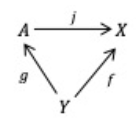
\includegraphics[width=1in]{images/image.PNG}
  \centering
 % \caption{Vertical angles.}
  %\label{fig:vert}
\end{figure}


Prove that $f$ is continuous if and only if $g$ is continuous.

Proof: Let $X_{\tau}$, $Y_{\nu}$ be topological spaces and $A$ a subspace of $X$. Let $f: Y \to X$ with $f(Y) \subseteq A$, and $g: Y \to A$ be such that $j \circ g = f$ where $j$ is the inclusion map of $A$ into $X$. 

First assume that $f$ is $(\nu - \tau)$ continuous. That is, for some $\tau$-open set $B$, we have that $f^{-1}(B)$ is a $\nu$-open subset of $Y$. Recall from a previous homework assignment that the inclusion map is continuous, and so $j^{-1}(B)$ is also a $\nu$-open subset of $Y$. Let $C = j^{-1}(B)$ and notice
\[f^{-1}(B) = (j \circ g)^{-1}(B)\]
\[= g^{-1}(j^{-1}(B))\]
\[f^{-1}(B) = g^{-1}(C)\]
Since $f^{-1}(B)$ is $\nu$-open, we have that $g^{-1}(C)$ is also $\nu$-open, so by definition, $g$ is continuous. 

Now assume that $g$ is continuous. We wish to show that $f$ is continuous. Let $B$ be a $\tau$-open set. Then since $j$ is continuous, we have that $j^{-1}(B)$ is $\tau_A$-open. And since $g$ is continuous, we have that $g^{-1}(j^{-1}(B))$ is $\nu$-open. Notice that
\[g^{-1}(j^{-1}(B)) = (j \circ g)^{-1}(B) = f^{-1}(B)\]
Thus, $f^{-1}(B)$ is $\nu$-open, and so by definition, $f$ is continuous.


\item Let $X$ be a set and let $A$ be a subset of $X$. Describe the closure of $A$ when $X$ has the following topologies:
\begin{enumerate}
\item the discrete topology, $\mathcal{D}$.

Since the discrete topology contains all subsets of X, we have that every $\mathcal{D}$-open set is also $\mathcal{D}$-closed, since for some $\mathcal{D}$ open set $B$, we have that $X \setminus B \subseteq X $, so $X \setminus B \in \mathcal{D}$. 

Thus, since $\mathcal{D}$ contains every subset of $X$, we have that $A \in \mathcal{D}$, and thus, $A$ is both $\mathcal{D}$-open and closed, so Cl($A$) =  $A$.


\item the indiscrete topology, $\mathcal{I}$.

Since the indiscrete topology contains only the empty set and $X$, i.e. $\mathcal{I} = \{\emptyset, X\}$. So the set of all $\mathcal{I}$-closed sets is also $\{\emptyset, X\}$ since $X \setminus X = \emptyset$ and $X \setminus \emptyset = X$. And so, the "smallest" $\mathcal{I}$ closed set that contains $A$ is $X$. Thus, Cl($A$) = $X$.


\item the finite complement topology, $\mathcal{FC}$.

If $A = \emptyset$, or $A = X$, by definition, $A$ is closed, so $\text{Cl}(A) = A$. If $A$ is a finite set, then we have that $A$ is also closed. To see this, let $A$ be a finite set. That is, $A \sim \{1,2,\ldots,n\}$ for some natural number $n$. We want to show that $A$ is closed. If $A$ is closed, then $X \setminus A$ would be open. That is, we want $X \setminus (X \setminus A)$ to be finite. Notice that
\[X \setminus (X \setminus A) = A\]
is finite by assumption. Thus, if $A$ is a finite set, then Cl($A$) = $A$.
\newline

If $A$ is not finite, then we have that Cl($A$) = $X$ since the smallest set that contains $A$ that is $\mathcal{FC}$ closed is $X$.
\end{enumerate}

\item Let $X_{\tau}$ be a topological space and let $A$ and $B$ be subsets of $X$. Denote the closure of a subset $S$ of $B$ with respect to the subspace topology on $B$ by $\text{Cl}_{\tau_B}(S)$. This is the smallest $\tau_B$-closed set containing $S$.
\begin{enumerate}
\item Show that $\text{Cl}_{\tau_B}(A\cap B)\subseteq \text{Cl}(A)\cap B$, where $\text{Cl}(A)$ refers to the closure of $A$ in $X$.

Proof: First consider the case where $A \cap B = \emptyset$. Then $\text{Cl}_{\tau_B}(A \cap B) = \emptyset \subseteq \text{Cl}(A) \cap B$.

Now consider the case where $A \cap B \neq \emptyset$. Then $\text{Cl}_{\tau_B}(A \cap B) \neq \emptyset$.
Let $x \in \text{Cl}_{\tau_B}(A \cap B)$. 
Since $\text{Cl}_{\tau_B}(A \cap B)$ is the smallest $\tau_B$-closed set containing $A \cap B$, we have that $x \in A \cap B$. 
By definition of set intersection, we have that $x \in A$ and $x \in B$. 

By definition, $\text{Cl}(A)$ is the smallest $\tau$-closed set containing $A$, so we have that $x \in \text{Cl}(A)$. And by definition of set intersection, since $x$ is an element of both $B$ and $\text{Cl}(A)$, we have that
\[x \in \text{Cl}(A) \cap B\]
Thus,
\[\text{Cl}_{\tau_B}(A \cap B) \subseteq \text{Cl}(A) \cap B\]

\item Give an example in which $\text{Cl}_{\tau_B}(A\cap B)$ is a proper subset of $\text{Cl}(A)\cap B$.

Let $X = \{1,2,3\}$ and $\tau = \{\emptyset, X, \{1\}, \{2\}, \{1,2\}\}$, and let $A = \{1,2\}$ and $B = \{3\}$. Consider the subspace topology on $B$:
\[\tau_B = \{\emptyset, \{3\}\}\]
and note that the set of $\tau_B$-closed sets are 
\[\{\emptyset, \{3\}\}\]
and the set of $\tau$-closed sets are
\[\{\emptyset, X, \{2,3\}, \{1,3\}, \{3\}\}\]
Now notice that 
\[A \cap B = \emptyset\]
so
\[\text{Cl}_{\tau_B}(A \cap B) = \emptyset\]
And notice that
\[\text{Cl}(A) = X\]
Then we have
\[\text{Cl}(A) \cap B = X \cap \{3\} = \{3\}\]

Clearly,
\[\text{Cl}_{\tau_B}(A \cap B) \subset \text{Cl}(A) \cap B\]
\end{enumerate}

\end{enumerate}

\end{document}
